\chapter{Erfelijkheid en kenmerken}\label{ch:g9:heredity-and-traits}

Familiefoto's zijn biologische gegevens. De kin van oma bij
de peuter, de krullen van de moeder bij geen van beide
kinderen, de ene broer lang en de andere niet --- gelijkenis
loopt in families, en verschil ook. Dit boek leunt al jaren
op dat feit (het veulen van
\cref{rem:g4:animal-reproduction:mix}, de broers en zussen van
\cref{prop:g8:sexual-reproduction:shuffle}); het
openingshoofdstuk van dit jaar bestudeert het eindelijk: wat
wordt er precies geërfd, wat niet, en wat mogen we uit de
patronen van familiegelijkenis concluderen?

\begin{omfigure}
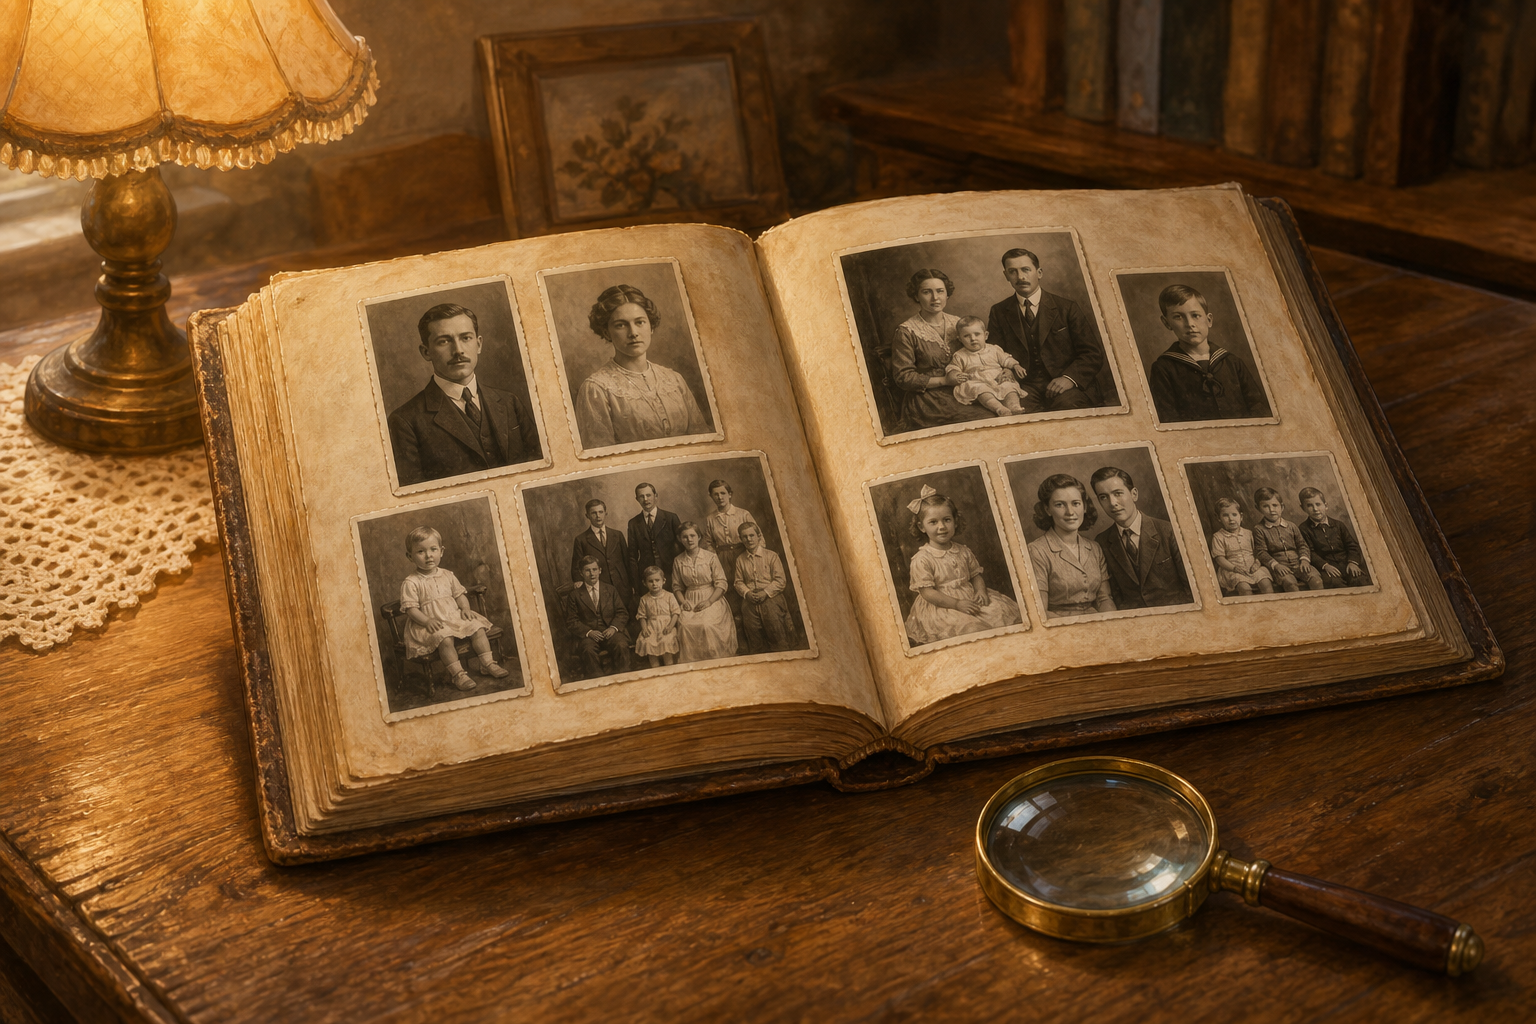
\includegraphics[width=0.62\linewidth]{images/book1/ai/g9-family-album.png}

{\small Biologische gegevens, in sepia: gelijkenis en
verschil, van generatie op generatie.}
\end{omfigure}

\section{Kenmerken, en waar ze vandaan komen}

\begin{definition}[Kenmerken]\label{def:g9:heredity-and-traits:traits}
Een \emph{kenmerk}\index{kenmerk} is elke beschrijfbare
eigenschap van een individu: oogkleur, bloedgroep, de vorm
van een oorlel, lengte, een zangstem, een litteken. De hele
verzameling kenmerken van een individu wordt door twee
werkingen gebouwd: wat \emph{geërfd} is, en wat de
\emph{\omterm{def:g6:exploring-our-environment:components}{omgeving} en het leven} eraan toevoegden (de wereld van
\cref{def:g4:adapted-to-their-world:adaptation}, werkend op
één lichaam).
\end{definition}

\begin{definition}[Erfelijkheid]\label{def:g9:heredity-and-traits:heredity}
\emph{Erfelijkheid}\index{erfelijkheid} is het doorgeven van
\omterm{def:g9:heredity-and-traits:traits}{kenmerken} van ouders aan nakomelingen via de voortplanting
--- via, zoals \cref{ch:g8:sexual-reproduction} liet zien,
twee losse cellen. \omterm{def:g9:heredity-and-traits:traits}{Kenmerken} die langs die weg overgaan zijn
\emph{erfelijk}\index{erfelijk kenmerk}: oogkleur en
bloedgroep wel; littekens en gaatjes in de \omterm{def:g1:the-five-senses:sense}{oren} niet, hoe
lang ook gedragen. De sorteertoets zijn de \omterm{def:g8:sexual-reproduction:gametes}{geslachtscellen}:
wat twee cellen niet kunnen dragen, kan geen familie doorgeven.
\end{definition}

\begin{example}[Een familiealbum sorteren]\label{ex:g9:heredity-and-traits:album}
De foto's van opa: zijn karakteristieke \omterm{def:g1:the-five-senses:sense}{neus} --- \omterm{def:g9:heredity-and-traits:heredity}{erfelijk},
daar is hij weer, bij de tante en bij de neef; zijn verweerde
boerenkleur --- verworven, zijn kantoorwerkende kleinzoon
mist hem; zijn lengte --- deels allebei, want de kleinzoon
steekt op hetzelfde postuur boven hem uit, gevoed door
rijkere jaren (\cref{prop:g3:balanced-diet:jobs}); zijn
vioolspel --- als vaardigheid niet \omterm{def:g9:heredity-and-traits:heredity}{erfelijk}
(\cref{ex:g8:nervous-communication:juggler}: synapsen worden
getraind, niet doorgegeven), al vertelt de muzikale familie
ons dat er iets subtielers meegaat in wat wordt doorgegeven:
misschien aanleg, nooit de getrainde bedrading zelf.
\end{example}

\begin{proposition}[Geërfd en verworven]\label{prop:g9:heredity-and-traits:sorting}
De twee werkingen laten zich op drie toetsen scheiden:
\begin{enumerate}
  \item \emph{familiepatroon}: erfelijke \omterm{def:g9:heredity-and-traits:traits}{kenmerken} keren in de
        \omterm{def:g6:classification-kinship:tree}{stamboom} terug langs de lijnen van de voortplanting;
        verworven \omterm{def:g9:heredity-and-traits:traits}{kenmerken} volgen levens (alle zeelieden
        verweerd, wie hun ouders ook waren);
  \item \emph{van het begin af aanwezig}: de bloedgroep ligt
        bij de \omterm{def:g5:flower-to-fruit:steps}{bevruchting} vast; de kleur en de vaardigheid
        worden daarna opgebouwd;
  \item \emph{doorgeven}: kinderen van geamputeerden hebben
        hun \omterm{def:g1:my-body:parts}{ledematen}; kinderen van bodybuilders beginnen
        ongetraind. Verworven \omterm{def:g9:heredity-and-traits:traits}{kenmerken} sterven met wie ze
        verwierf --- de \omterm{def:g8:sexual-reproduction:gametes}{geslachtscellen} dragen ze niet.
\end{enumerate}
De meeste zichtbare \omterm{def:g9:heredity-and-traits:traits}{kenmerken} --- lengte, bouw, zelfs
temperament --- zijn uit beide werkingen geweven: een geërfde
marge, met leven ingevuld.
\end{proposition}
\admitted

\section{Familiepatronen lezen}

\begin{example}[Kenmerken die overslaan]\label{ex:g9:heredity-and-traits:skip}
Sommige patronen verbazen op het eerste gezicht: twee
bruinogige ouders met een blauwogig kind; een \omterm{def:g9:heredity-and-traits:traits}{kenmerk} van oma
dat bij geen enkel kind verschijnt en toch bij een kleinkind
terugkomt. Overslaan is gewoon, en het draagt een zware
conclusie: een ouder kan \emph{doorgeven wat hij niet toont}.
De instructies voor het \omterm{def:g9:heredity-and-traits:traits}{kenmerk} reisden verborgen door een
generatie --- dus wat geërfd wordt is niet het \omterm{def:g9:heredity-and-traits:traits}{kenmerk} zelf,
maar iets dat het \emph{bepaalt}, ongezien draagbaar.
\end{example}

\begin{proposition}[Wat de patronen ons doen concluderen]\label{prop:g9:heredity-and-traits:conclusions}
Drie conclusies, elk door een waarneming afgedwongen:
\begin{enumerate}
  \item omdat verworven \omterm{def:g9:heredity-and-traits:traits}{kenmerken} niet overgaan, moet wat
        overgaat uit \emph{bepalers} bestaan --- instructies
        om \omterm{def:g9:heredity-and-traits:traits}{kenmerken} te bouwen, niet de \omterm{def:g9:heredity-and-traits:traits}{kenmerken} zelf;
  \item omdat \omterm{def:g9:heredity-and-traits:traits}{kenmerken} generaties overslaan, kunnen de
        bepalers \emph{gedragen worden zonder te tonen}: elk
        individu draagt meer dan het laat zien;
  \item omdat elk kind van beide ouders ontvangt via twee
        \omterm{def:g8:sexual-reproduction:gametes}{geslachtscellen}
        (\cref{prop:g8:sexual-reproduction:core}), draagt elke
        ouder een \emph{selectie} van zijn bepalers bij --- en
        de selecties verschillen van kind tot kind, anders
        zouden broers en zussen gelijk zijn
        (het schudden van
        \cref{prop:g8:sexual-reproduction:shuffle}, nu
        gelokaliseerd: het is een schudden \emph{van bepalers}).
\end{enumerate}
\end{proposition}
\admitted

\begin{remark}[De vraag die dit stelt]\label{rem:g9:heredity-and-traits:question}
Het familiealbum heeft ons in een prachtige vraag gedreven.
Ergens in het bijna-niets van een \omterm{def:g8:reproductive-systems:male}{zaadcel}
(\cref{ex:g8:reproductive-systems:sperm} --- een
samengepakte kern en een \omterm{def:g1:animals-around-us:parts}{staart}) reizen instructies voor een
\omterm{def:g1:the-five-senses:sense}{neus}, een bloedgroep, een oogkleur mee --- ongetoond te
dragen, per helft te selecteren, leesbaar voor het groeiende
lichaam. \emph{Waar zitten ze, en waarvan zijn ze gemaakt?}
De anatomie van de \omterm{def:g8:reproductive-systems:male}{zaadcel} wijst het antwoord al aan: alles
wat de vader stuurt past in een kern
(\cref{rem:g5:first-look-at-cells:nucleus} beloofde dat die
plek ertoe deed). De volgende twee hoofdstukken openen hem.
\end{remark}

\begin{method}[Een kenmerk keuren]\label{met:g9:heredity-and-traits:audit}
Loop bij elk \omterm{def:g9:heredity-and-traits:traits}{kenmerk} de drie toetsen af:
\begin{enumerate}
  \item zet het uit op de \omterm{def:g6:classification-kinship:tree}{stamboom}: volgt het de lijnen van de
        voortplanting, of levens en gewoonten?
  \item dateer het: van het begin af vast, of onderweg
        opgebouwd?
  \item pas de geslachtsceltoets toe: zouden twee cellen het
        kunnen dragen? (een litteken niet; een bloedgroep wel);
  \item oordeel: geërfd, verworven, of --- het vaakst --- een
        geërfde marge, ingeleefd.
\end{enumerate}
\end{method}

\section{Oefeningen}

\begin{exercise}[$\star$]\label{exo:g9:heredity-and-traits:1}
Definieer \omterm{def:g9:heredity-and-traits:traits}{kenmerk} en \omterm{def:g9:heredity-and-traits:heredity}{erfelijkheid}, en geef de sorteertoets in
één zin.
\end{exercise}

\begin{exercise}[$\star$]\label{exo:g9:heredity-and-traits:2}
Rangschik: bloedgroep; een gaatje in het \omterm{def:g1:the-five-senses:sense}{oor}; sproeten; vlot
Frans; de vorm van een oorlel.
\end{exercise}

\begin{exercise}[$\star$]\label{exo:g9:heredity-and-traits:3}
Noem de drie toetsen van
\cref{prop:g9:heredity-and-traits:sorting}.
\end{exercise}

\begin{exercise}[$\star$]\label{exo:g9:heredity-and-traits:4}
Waarom beginnen kinderen van bodybuilders ongetraind? Wat
laat dat zien?
\end{exercise}

\begin{exercise}[$\star$]\label{exo:g9:heredity-and-traits:5}
Wat bewijst een overslaand \omterm{def:g9:heredity-and-traits:traits}{kenmerk} dat een ouder kan?
\end{exercise}

\begin{exercise}[$\star$]\label{exo:g9:heredity-and-traits:6}
Waarom moet wat geërfd wordt uit bepalers bestaan en niet uit
\omterm{def:g9:heredity-and-traits:traits}{kenmerken}? Eén zin.
\end{exercise}

\begin{exercise}[$\star\star$]\label{exo:g9:heredity-and-traits:7}
De kleinzoon werd op hetzelfde postuur langer. Ontwar de twee
werkingen in die zin.
\end{exercise}

\begin{exercise}[$\star\star$]\label{exo:g9:heredity-and-traits:8}
Leg in de taal van bepalers uit waarom broers en zussen
verschillen --- en waarom eeneiige tweelingen
(\cref{exo:g8:from-egg-to-birth:10}) dat niet doen.
\end{exercise}

\begin{exercise}[$\star\star$]\label{exo:g9:heredity-and-traits:9}
Pas \cref{met:g9:heredity-and-traits:audit} toe op: (a) het
vroege grijs dat in een familie terugkeert; (b) het
uithoudingsvermogen van een voetballer.
\end{exercise}

\begin{exercise}[$\star\star$]\label{exo:g9:heredity-and-traits:10}
Het vioolgeval: wat zou de muzikale familie kunnen doorgeven,
als het nooit de getrainde vaardigheid is? Onderscheid
zorgvuldig.
\end{exercise}

\begin{exercise}[$\star\star$]\label{exo:g9:heredity-and-traits:11}
Twee bruinogige ouders, een blauwogig kind --- en de buurman
twijfelt aan de familie. Verdedig de familie met de logica
van \cref{ex:g9:heredity-and-traits:skip}.
\end{exercise}

\begin{exercise}[$\star\star\star$]\label{exo:g9:heredity-and-traits:12}
Beredeneer alleen uit de anatomie van de \omterm{def:g8:reproductive-systems:male}{zaadcel}
(\cref{ex:g8:reproductive-systems:sperm}) waar de bepalers van
de vader moeten zitten --- en welke omvang dat voor de
instructies van een heel mens impliceert.
\end{exercise}

\section{Probleem: De dorpsgenealoog}

\begin{problem}[{Weekendprobleem --- drie generaties,
één kenmerkenregister}]\label{pb:g9:heredity-and-traits:1}
Een dorpsgenealoog schrijft bij de stambomen van de parochie
\omterm{def:g9:heredity-and-traits:traits}{kenmerken} bij: de ``kapelkin'' (een karakteristieke kin die al
een eeuw terugkeert), linkshandigheid, de meelhoest van de
bakkers, bloedgroepen uit het donorregister, en de verweerde
gezichten van de herders.

\medskip\noindent\textbf{Deel I --- Het register
sorteren.}
\begin{enumerate}
  \item Sorteer de vijf \omterm{def:g9:heredity-and-traits:traits}{kenmerken} met
        \cref{met:g9:heredity-and-traits:audit}, met bij elk
        de beslissende toets.
  \item De hoest volgt de bakkerij, niet de familie: erin
        trouwen brengt hem mee, wegverhuizen raakt hem kwijt.
        Welke toets is dit, in actie?
  \item De kapelkin slaat in twee takken de middelste
        generatie over. Trek de conclusie die dat afdwingt.
  \item Bloedgroepen verrassen het register soms: een kind met
        groep O van ouders met groep A en groep B. Wat moet
        elke ouder gedragen hebben?
\end{enumerate}

\medskip\noindent\textbf{Deel II --- De lezing met
bepalers.}
\begin{enumerate}[resume]
  \item Herschrijf de eeuw van de kin in de taal van bepalers:
        wat reisde er werkelijk vier generaties omlaag, en in
        welke voertuigen
        (\cref{def:g9:heredity-and-traits:heredity})?
  \item Waarom verschillen de neven en nichten met de kin in
        al het overige? Lokaliseer het schudden.
  \item De genealoog vindt in een eeuw geen enkel geval van
        een litteken, een ambacht of een taal die aan een
        pasgeborene overgaat. Formuleer de algemene regel, en
        haar reden op mechanismeniveau.
  \item De tweeling van één familie komt overeen tot en met de
        kin en verder. Wat concludeert het register over hun
        begin
        (\cref{rem:g5:human-reproduction:twins})?
\end{enumerate}

\medskip\noindent\textbf{Deel III --- De lezing.}
\begin{enumerate}[resume]
  \item De genealoog spreekt: ``de parochie geeft twee erfenissen
        door --- de ene via \omterm{def:g8:sexual-reproduction:gametes}{geslachtscellen}, de andere via
        samenleven.'' Wijs de vijf \omterm{def:g9:heredity-and-traits:traits}{kenmerken} van het register
        aan de twee kanalen toe.
  \item ``Ieder van ons toont minder dan hij draagt.''
        Verdedig dat twee keer uit het register.
  \item Een toehoorder vraagt wat de instructies van het
        geslachtscelkanaal fysiek zijn. Geef het eerlijke
        antwoord van \cref{rem:g9:heredity-and-traits:question}
        --- plaats bekend, inhoud volgend hoofdstuk.
  \item Sluit de lezing af met het eenregelige oordeel van de
        keuring over het gewoonste geval: de meeste \omterm{def:g9:heredity-and-traits:traits}{kenmerken}
        zijn \emph{wat}, geleefd \emph{hoe}?
\end{enumerate}
\end{problem}
